\section{Probability}
\subsection{Random Variables}
\begin{itemize}
    \item Values depend on outcomes of a random phenomenon
    \item Random variable $X$ is a variable that takes a numerical value $x$, which depends on a random experiment
    \item \textbf{Discrete:} $X$ takes any of a finite set of values ${1.5, 2.123, 6.2, 10}$
    \item \textbf{Continous:} $X$ takes any alue of an uncountable range e.g. real numbers from an interval
\end{itemize}
\textbf{Best we can know}
\begin{itemize}
    \item All possible values
    \item Probability of each value
\end{itemize}
E.g. The discrete random variable $X$ is the number observed when rolling a fair dice.\\ 
$Pr(X=x)$ / $P(x)$: $1/6$ for each possible value (the probability that the random variable X takes the value x)

\subsubsection{Two random variables}
\textbf{Joint Probability}
\begin{itemize}
    \item Joint Properties of two random variables
    \item Defined by the Joint Probability Mass Function
\end{itemize}
E.g. Dice1 = 5 AND Dice2 = 4\\
$P_{XY}(5,4) = 1/36$\\ 
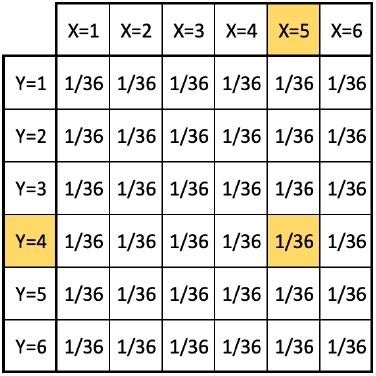
\includegraphics[width=0.5\linewidth]{./img/joint_probability.png} \\
\textbf{Correlated random Variables}
\begin{itemize}
    \item There are events that are not independant
    \item Such random variables are correlated
    \item $X$: observe clouds (0=no, 1=small, 2=big)
    \item $Y$: observe rain (0=no, 1=light, 2=moderate, 3=heavy)
\end{itemize}

\subsubsection{Join Probability/ Independant random Variables}
\begin{itemize}
    \item Joint Probability is the product of the individual probabilities
\end{itemize}
$P(X,Y) = P(X) \cdot P(Y)$ (only if independant)\\ 
$P(X,Y,Z) = P(X) \cdot P(Y) \cdot P(Z)$ (only if independant)

\subsubsection{Conditional Probability}
\begin{itemize}
    \item One variable is no longer random
    \item X is observed, its value is fixed
    \item Calculate the probabilities of Y given X: $P(Y | X)$
\end{itemize}
$P(X, Y) = P(X | Y) \cdot P(Y)$\\ 
$P(X, Y) = P(Y | X) \cdot P(X)$\\
$P(Y | X) = \frac{P(X,Y)}{P(X)}$

\subsubsection{Marginal Probability}
\begin{itemize}
    \item What is the general approach to recover the PMF Pr(X=x) of one random variable, given the joint probability Pr(X,Y) ?
    \item Man kann immer die Summen bilden (siehe Beispiel anhand Tabelle)
    \begin{itemize}
        \item $P(X=1) = Y(1) + Y(2) + Y(3) + Y(4) + Y(5) + Y(6) = 6/36 = 1/6$
    \end{itemize}
    \item Marginal Distribution = Summe einer Dimension (X oder Y)
\end{itemize}

\subsubsection{Bayes Rule}
$P(X|Y) \cdot P(Y) = P(Y|X) \cdot P(X)$\\ 
Therefore:\\
$P(Y|X) = \frac{P(X|Y) \cdot P(Y)}{P(X)}$

\subsubsection{Probability Mass Function (PMF)}
\begin{minipage}{0.6 \linewidth}
The PMF of a discrete random variable is a function $f(x)$ that provides the probability for each value $x$ of a discrete random variable $X$.\\
A PMF specifies a (discrete) \textbf{Probability Distribution} (de: Wahrscheinlichkeitsverteilung). (but often the two terms are used as synonyms.)\\
\textbf{Aus Übung:} density = dursch. hits / nr of samples. Für Warscheinlichkeit Fläche unter der Kurve ausrechnen. Also z.b. Interval [-4,-1] und Density 0.1 = 0.1*3=30\%
\end{minipage}
\begin{minipage}{0.4 \linewidth}
\centering
Graph of a PMF (dice) $f(x)$:\\
\begin{tikzpicture}
    \begin{axis}[
    width=\textwidth,
    height=3cm,
    xmin = 0, xmax = 6,
    ymin = 0, ymax = 1,
    ytick={1/6,1},
    yticklabels={$\frac{1}{6}$,1},
    xtick={1,2,3,4,5,6},
    axis y line=left,
    axis x line=bottom,
    xlabel=$x$, ylabel=$f(x)$, 
    ]
        \addplot[black, only marks] coordinates {
          (1, 1/6)
          (2, 1/6)
          (3, 1/6)
          (4, 1/6)
          (5, 1/6)
          (6, 1/6)
        };
    \end{axis}
\end{tikzpicture}
\end{minipage}